\documentclass[a4paper,10pt]{article}\usepackage[]{graphicx}\usepackage[]{color}
%% maxwidth is the original width if it is less than linewidth
%% otherwise use linewidth (to make sure the graphics do not exceed the margin)
\makeatletter
\def\maxwidth{ %
  \ifdim\Gin@nat@width>\linewidth
    \linewidth
  \else
    \Gin@nat@width
  \fi
}
\makeatother

\definecolor{fgcolor}{rgb}{0.345, 0.345, 0.345}
\newcommand{\hlnum}[1]{\textcolor[rgb]{0.686,0.059,0.569}{#1}}%
\newcommand{\hlstr}[1]{\textcolor[rgb]{0.192,0.494,0.8}{#1}}%
\newcommand{\hlcom}[1]{\textcolor[rgb]{0.678,0.584,0.686}{\textit{#1}}}%
\newcommand{\hlopt}[1]{\textcolor[rgb]{0,0,0}{#1}}%
\newcommand{\hlstd}[1]{\textcolor[rgb]{0.345,0.345,0.345}{#1}}%
\newcommand{\hlkwa}[1]{\textcolor[rgb]{0.161,0.373,0.58}{\textbf{#1}}}%
\newcommand{\hlkwb}[1]{\textcolor[rgb]{0.69,0.353,0.396}{#1}}%
\newcommand{\hlkwc}[1]{\textcolor[rgb]{0.333,0.667,0.333}{#1}}%
\newcommand{\hlkwd}[1]{\textcolor[rgb]{0.737,0.353,0.396}{\textbf{#1}}}%
\let\hlipl\hlkwb

\usepackage{framed}
\makeatletter
\newenvironment{kframe}{%
 \def\at@end@of@kframe{}%
 \ifinner\ifhmode%
  \def\at@end@of@kframe{\end{minipage}}%
  \begin{minipage}{\columnwidth}%
 \fi\fi%
 \def\FrameCommand##1{\hskip\@totalleftmargin \hskip-\fboxsep
 \colorbox{shadecolor}{##1}\hskip-\fboxsep
     % There is no \\@totalrightmargin, so:
     \hskip-\linewidth \hskip-\@totalleftmargin \hskip\columnwidth}%
 \MakeFramed {\advance\hsize-\width
   \@totalleftmargin\z@ \linewidth\hsize
   \@setminipage}}%
 {\par\unskip\endMakeFramed%
 \at@end@of@kframe}
\makeatother

\definecolor{shadecolor}{rgb}{.97, .97, .97}
\definecolor{messagecolor}{rgb}{0, 0, 0}
\definecolor{warningcolor}{rgb}{1, 0, 1}
\definecolor{errorcolor}{rgb}{1, 0, 0}
\newenvironment{knitrout}{}{} % an empty environment to be redefined in TeX

\usepackage{alltt}
\IfFileExists{upquote.sty}{\usepackage{upquote}}{}
\begin{document}

\section{Introduction}

\subsection{Background}
The core graphics system in R can been divided in to two main packages. The first package is the graphics package. It is older and it provides the original GRZ graphics system from S, sometimes referred to as ``traditional'' graphics. It is relatively fast and many other R packages build on top of it. The newer package is the grid package. It is actually slower but is has more flexibility and additional features compared to the graphics package. \\\\
A graph that is drawn using grid can been edited in many more ways than a graph that has been drawn using the basic graphics package. However, there is a new package, called gridGrahics, which allows us to convert a plot that has been drawn by the graphics package to an equivalent plot drawn by grid graphics. This means that the additional flexibility and features of grid become available for any plot drawn using the graphics package. 

\subsection{The \texttt{gridGraphic} package}
\texttt{gridGraphic} is like a 'translator' that translate the plot which been drawn by using the basic graphics package to the plot which been drawn by using grid package. 
The \texttt{gridGraphic} package has a main function called \texttt{grid.echo()}, which takes a recorded plot (or NULL for the current plot of the current graphic dervice) as an argument. Then it replicate the 
plot by using grid so that the user may edites the plot in more way than the plot drawn by bacis graphic package.
The following code provides a quick example. We generate 25 random numbers for x and y. First, we draw a scatter plot using the function plot() from the basic graphic package, then we redraw it using grid.echo() from the gridGraphic package with grid.
\begin{knitrout}
\definecolor{shadecolor}{rgb}{0.969, 0.969, 0.969}\color{fgcolor}\begin{kframe}
\begin{alltt}
\hlkwd{setwd}\hlstd{(}\hlnum{110}\hlstd{)}
\hlstd{x} \hlkwb{=} \hlkwd{runif}\hlstd{(}\hlnum{25}\hlstd{)}
\hlstd{y} \hlkwb{=} \hlkwd{runif}\hlstd{(}\hlnum{25}\hlstd{)}
\hlkwd{plot}\hlstd{(x,y,} \hlkwc{pch} \hlstd{=} \hlnum{16}\hlstd{)}
\hlkwd{grid.echo}\hlstd{()}
\end{alltt}
\end{kframe}
\end{knitrout}
\begin{figure}[h]
\begin{center}
  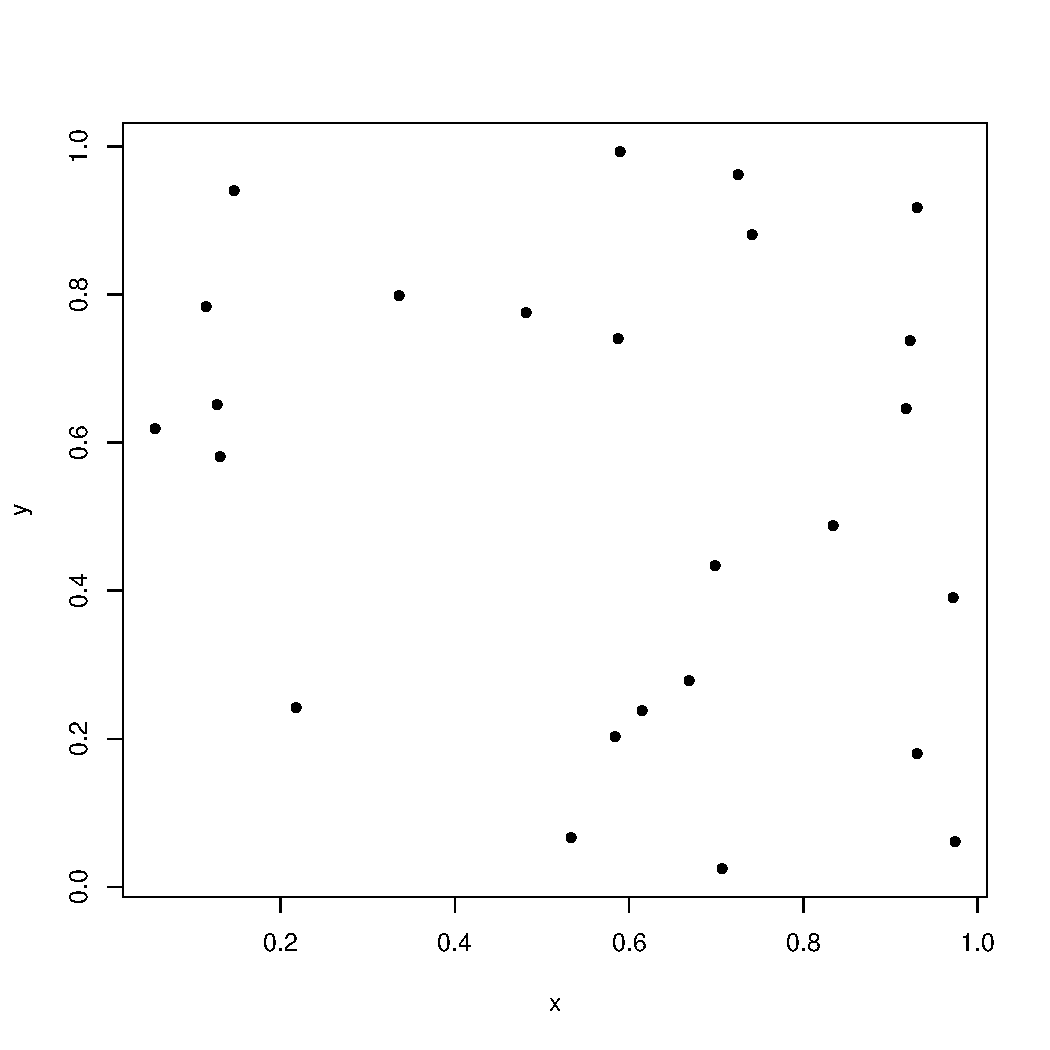
\includegraphics[height = 3.5cm, width = 5cm]{figure/basic.pdf}
  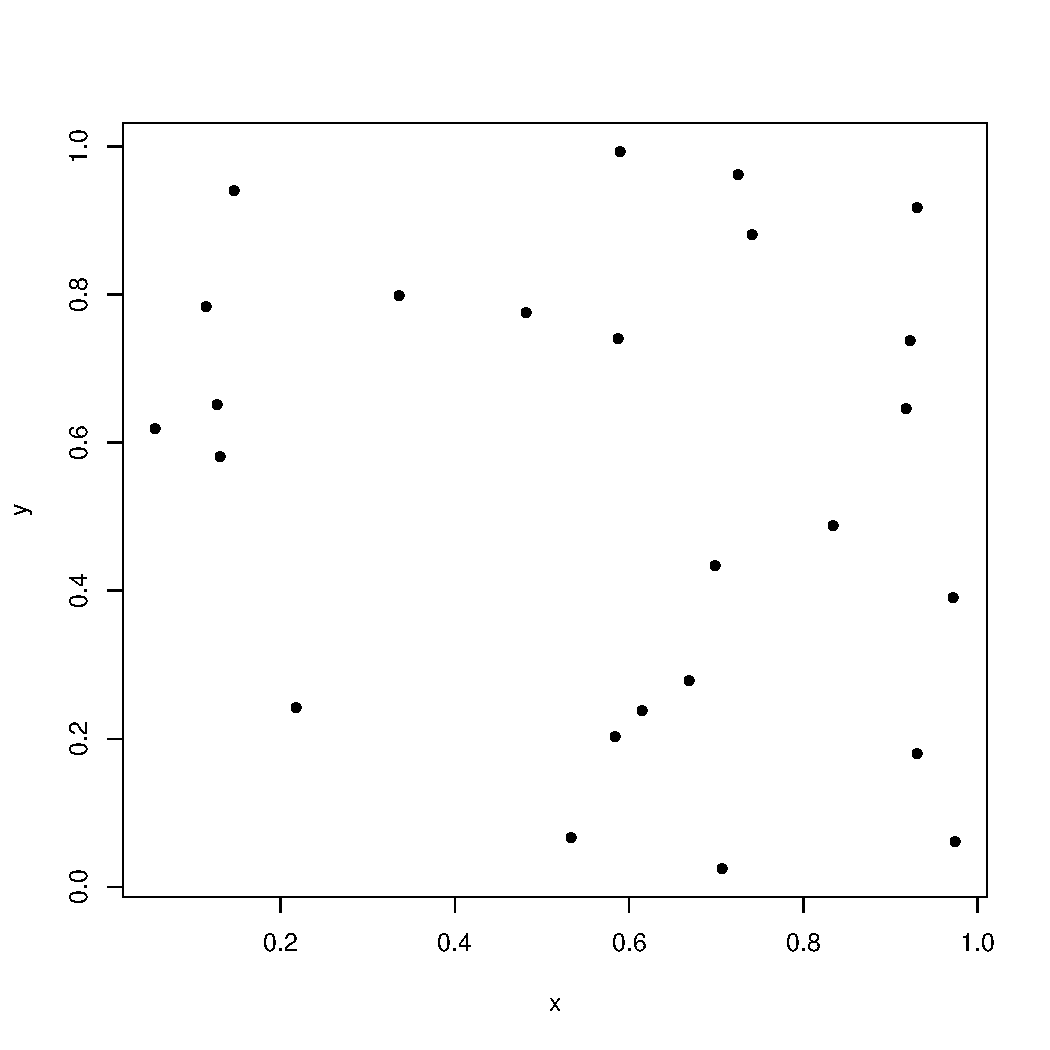
\includegraphics[height = 3.5cm, width = 5cm]{figure/echo.pdf}
  \caption{The left plot drawn by using plot(), the Right plot is redraw it by using grid.echo() on grid graphic system, overall, they are identical to each other}
  	\label{figure1}
\end{center}
\end{figure}
Alternatively, one example that shows the advantage of drawing the plot using grid rather than basic is that there is an object, called grid grobs, which recored a list of the details of each components of the plot that been drawn. The list of grobs can been seen by calling the function \texttt{grid.ls()}. \\
\begin{knitrout}
\definecolor{shadecolor}{rgb}{0.969, 0.969, 0.969}\color{fgcolor}\begin{kframe}
\begin{alltt}
\hlstd{graphics}\hlopt{-}\hlstd{background}
\hlstd{graphics}\hlopt{-}\hlstd{plot}\hlopt{-}\hlnum{1}\hlopt{-}\hlstd{points}\hlopt{-}\hlnum{1}
\hlstd{graphics}\hlopt{-}\hlstd{plot}\hlopt{-}\hlnum{1}\hlopt{-}\hlstd{bottom}\hlopt{-}\hlstd{axis}\hlopt{-}\hlstd{line}\hlopt{-}\hlnum{1}
\hlstd{graphics}\hlopt{-}\hlstd{plot}\hlopt{-}\hlnum{1}\hlopt{-}\hlstd{bottom}\hlopt{-}\hlstd{axis}\hlopt{-}\hlstd{ticks}\hlopt{-}\hlnum{1}
\hlstd{graphics}\hlopt{-}\hlstd{plot}\hlopt{-}\hlnum{1}\hlopt{-}\hlstd{bottom}\hlopt{-}\hlstd{axis}\hlopt{-}\hlstd{labels}\hlopt{-}\hlnum{1}
\hlstd{graphics}\hlopt{-}\hlstd{plot}\hlopt{-}\hlnum{1}\hlopt{-}\hlstd{left}\hlopt{-}\hlstd{axis}\hlopt{-}\hlstd{line}\hlopt{-}\hlnum{1}
\hlstd{graphics}\hlopt{-}\hlstd{plot}\hlopt{-}\hlnum{1}\hlopt{-}\hlstd{left}\hlopt{-}\hlstd{axis}\hlopt{-}\hlstd{ticks}\hlopt{-}\hlnum{1}
\hlstd{graphics}\hlopt{-}\hlstd{plot}\hlopt{-}\hlnum{1}\hlopt{-}\hlstd{left}\hlopt{-}\hlstd{axis}\hlopt{-}\hlstd{labels}\hlopt{-}\hlnum{1}
\hlstd{graphics}\hlopt{-}\hlstd{plot}\hlopt{-}\hlnum{1}\hlopt{-}\hlstd{box}\hlopt{-}\hlnum{1}
\hlstd{graphics}\hlopt{-}\hlstd{plot}\hlopt{-}\hlnum{1}\hlopt{-}\hlstd{xlab}\hlopt{-}\hlnum{1}
\hlstd{graphics}\hlopt{-}\hlstd{plot}\hlopt{-}\hlnum{1}\hlopt{-}\hlstd{ylab}\hlopt{-}\hlnum{1}
\end{alltt}
\end{kframe}
\end{knitrout}

As we see, the \texttt{grid.ls()} returns a list of grid grobs of the pervious plot that been redrawn by grid. there is one element called "graphics-plot-1-bottom-axis-labels-1" which is the element of the label of the bottom axis. There are several function on the \texttt{grid} package that used for mainpulate this grob. For example, if the user wants to rotate the labels of the bottom axis by 30 degrees and changes the color from default to orange, then the following code mainpulate this changes.

\begin{knitrout}
\definecolor{shadecolor}{rgb}{0.969, 0.969, 0.969}\color{fgcolor}\begin{kframe}
\begin{alltt}
\hlkwd{grid.edit}\hlstd{(}\hlstr{"graphics-plot-1-bottom-axis-labels-1"}\hlstd{,}
          \hlkwc{rot}\hlstd{=}\hlnum{30}\hlstd{,} \hlkwc{gp}\hlstd{=}\hlkwd{gpar}\hlstd{(}\hlkwc{col}\hlstd{=}\hlstr{"orange"}\hlstd{))}
\end{alltt}
\end{kframe}
\end{knitrout}

\begin{figure}[h]
\begin{center}
  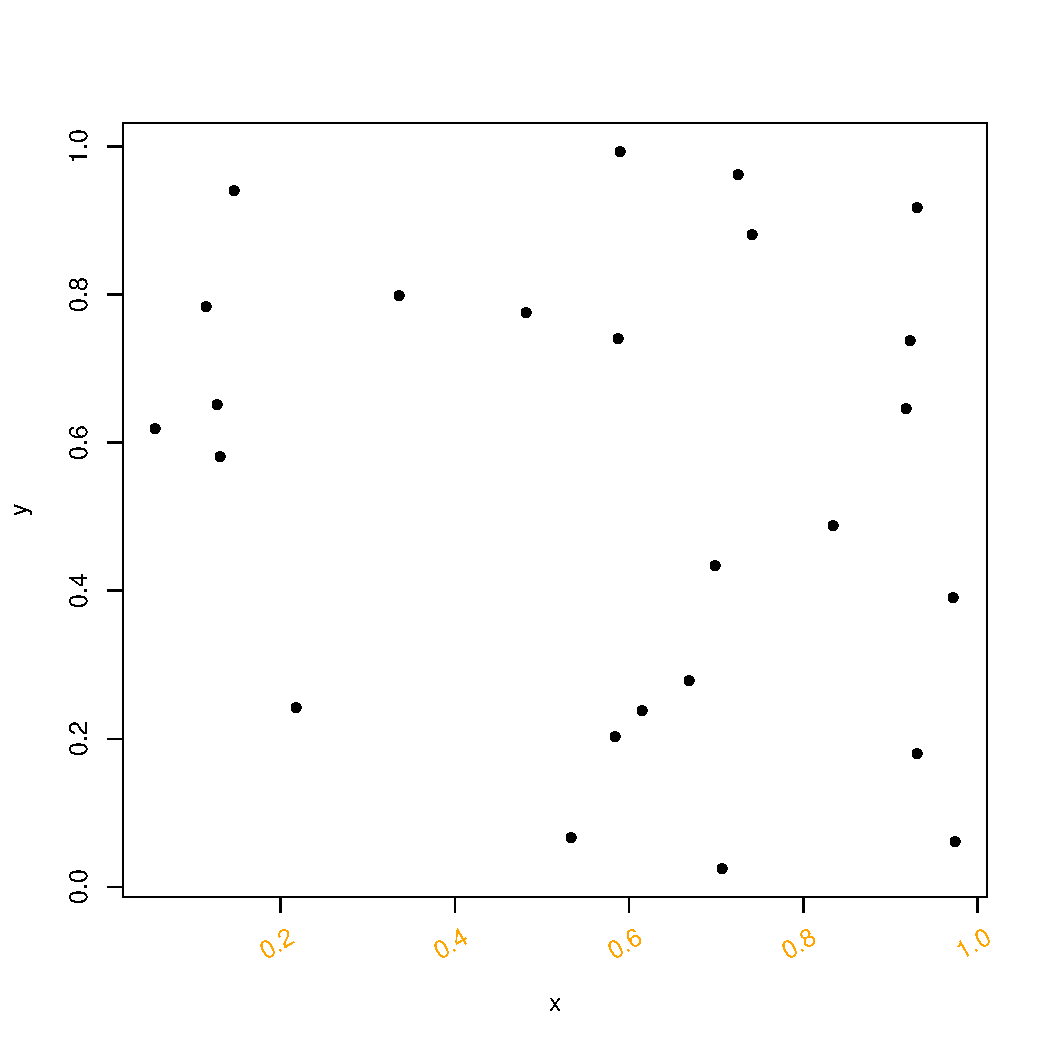
\includegraphics[height = 5cm, width = 6cm]{figure/gridedit.pdf}
  \caption{The angel and the color of the bottom axis of the previous plot been change by 30 degree and orange}
  	\label{figure3}
\end{center}
\end{figure}





\subsection{The problem}
The grid.echo() function can replicate most plots that are drawn by the graphics package. However, there are a few functions in the graphics package that grid.echo() cannot replicate. One such function is persp() which draws 3-dimemtional surfaces, the other one is the filled.contour(). This leads to the aim of this project. If we can draw a plot with persp() or filled.countour(), the result from calling grid.echo() is a blank screen 

\begin{knitrout}
\definecolor{shadecolor}{rgb}{0.969, 0.969, 0.969}\color{fgcolor}\begin{kframe}
\begin{alltt}
\hlstd{x} \hlkwb{<-} \hlstd{y} \hlkwb{<-} \hlkwd{seq}\hlstd{(}\hlopt{-}\hlnum{4}\hlopt{*}\hlstd{pi,} \hlnum{4}\hlopt{*}\hlstd{pi,} \hlkwc{len} \hlstd{=} \hlnum{27}\hlstd{)}
\hlstd{r} \hlkwb{<-} \hlkwd{sqrt}\hlstd{(}\hlkwd{outer}\hlstd{(x}\hlopt{^}\hlnum{2}\hlstd{, y}\hlopt{^}\hlnum{2}\hlstd{,} \hlstr{"+"}\hlstd{))}
\hlkwd{filled.contour}\hlstd{(}\hlkwd{cos}\hlstd{(r}\hlopt{^}\hlnum{2}\hlstd{)}\hlopt{*}\hlkwd{exp}\hlstd{(}\hlopt{-}\hlstd{r}\hlopt{/}\hlstd{(}\hlnum{2}\hlopt{*}\hlstd{pi)),} \hlkwc{frame.plot} \hlstd{=} \hlnum{FALSE}\hlstd{,} \hlkwc{plot.axes} \hlstd{= \{\})}
\end{alltt}
\end{kframe}
\end{knitrout}

\begin{figure}[h]
\begin{center}
  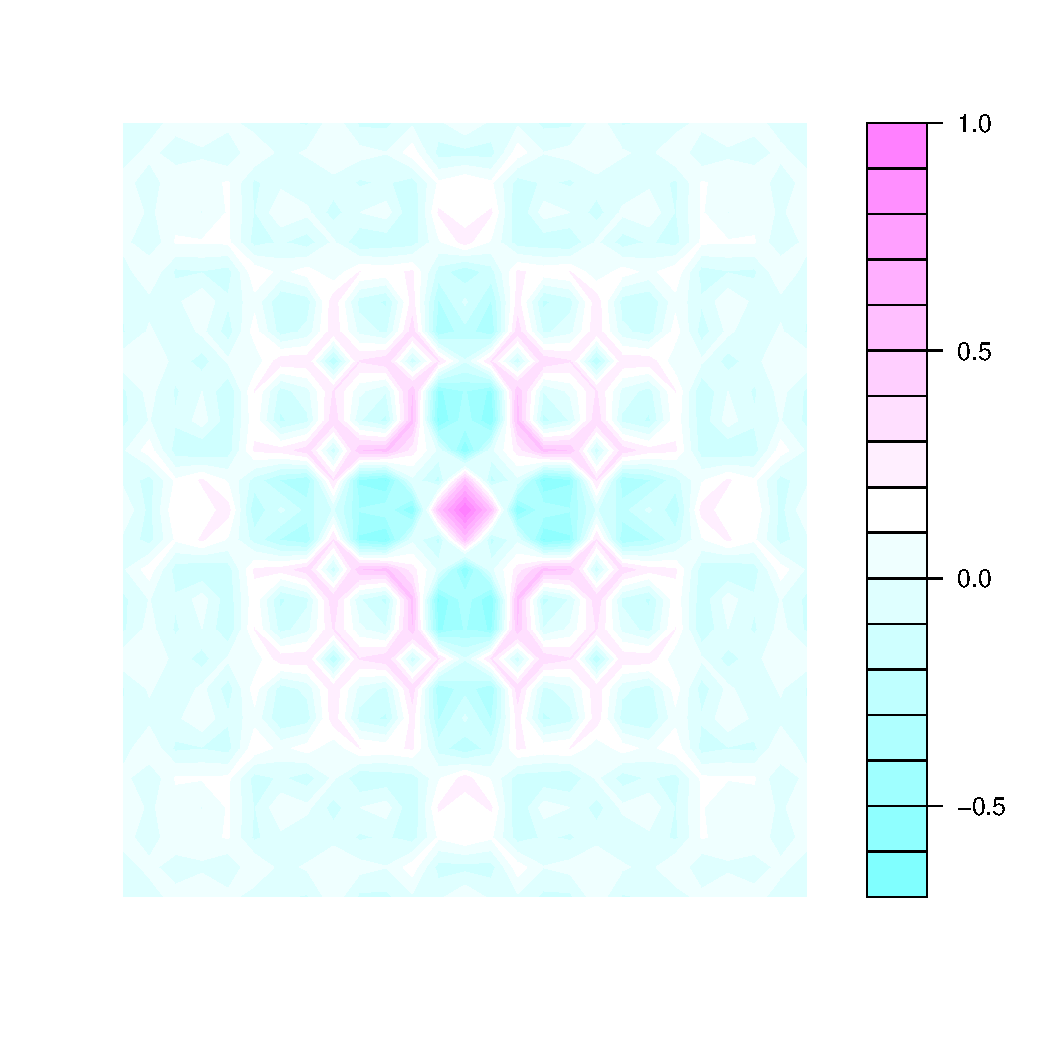
\includegraphics[height = 5cm, width = 6cm]{figure/filled-contour.pdf}
  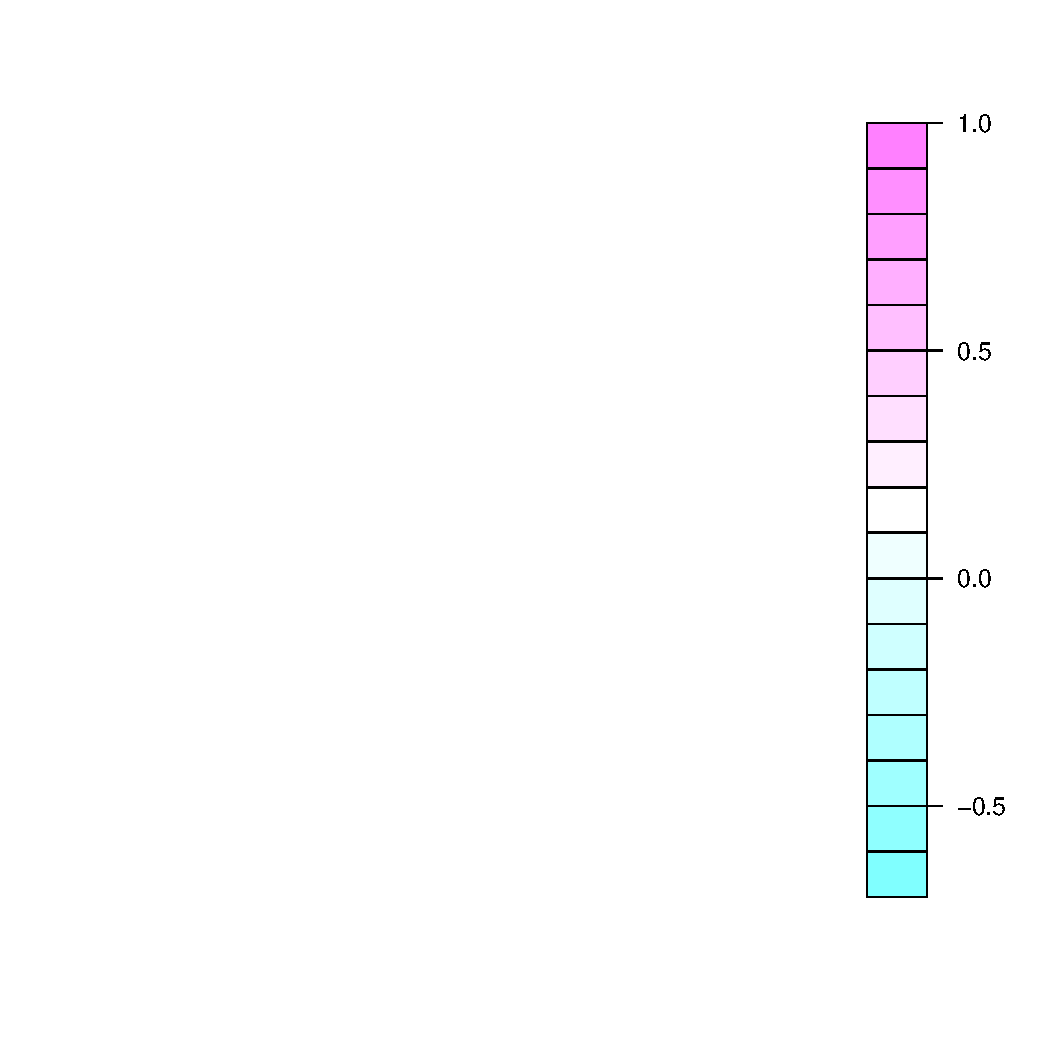
\includegraphics[height = 5cm, width = 6cm]{figure/filled-contour-gridecho.pdf}
  \caption{The left plot been drawn by using \texttt{filled.contour} and the right plot been redrawn by calling grid.echo(). There is a "blank" page on the right plot because the grid.echo cannot emulate filled.contour()}
  	\label{figure4}
\end{center}
\end{figure}

\subsection{Aim of this project}
The functions persp() and filled.contour() are wrote by C. However, it is very hard to debug and track the C code. One possible solution will be: 
1. read and understand the C code, do the direct translation from C code to R code.
2. ....


NOTE to Jason: explain how gridGraphics works first: graphics display list; gridGraphics implements an R version of each low-level C function on the display list (e.g., for C\_plot\_xy there is an R function called C\_plot\_xy in the gridGraphics package). THEN maybe write about 3D to 2D transformations, but only maybe.


\section{The graphics engine display list}
The information of evey plot drawn by R can be recorded. For example, In the simple \texttt{plot()} function, it is possible to obtain the parameters for x and y, even the label of the x-axis and y-axis.
This information is called the graphics engine display list. This is the list that contain the informations so that user can access and use for further work. In this paper, we use this graphics engine display list for replicate the persp() plot and contour() plot by using grid.

To access the graphics engine display list, the \texttt{recordPlot()} function been used. This is the function for saving the plot in an R object. 

\begin{knitrout}
\definecolor{shadecolor}{rgb}{0.969, 0.969, 0.969}\color{fgcolor}\begin{kframe}
\begin{alltt}
\hlkwd{plot}\hlstd{(cars}\hlopt{$}\hlstd{speed, cars}\hlopt{$}\hlstd{dist,} \hlkwc{col} \hlstd{=} \hlstr{'orange'}\hlstd{,}
      \hlkwc{pch} \hlstd{=} \hlnum{16}\hlstd{,} \hlkwc{xlab} \hlstd{=} \hlstr{'speed'}\hlstd{,} \hlkwc{ylab} \hlstd{=} \hlstr{'dist'}\hlstd{)}
\end{alltt}
\end{kframe}
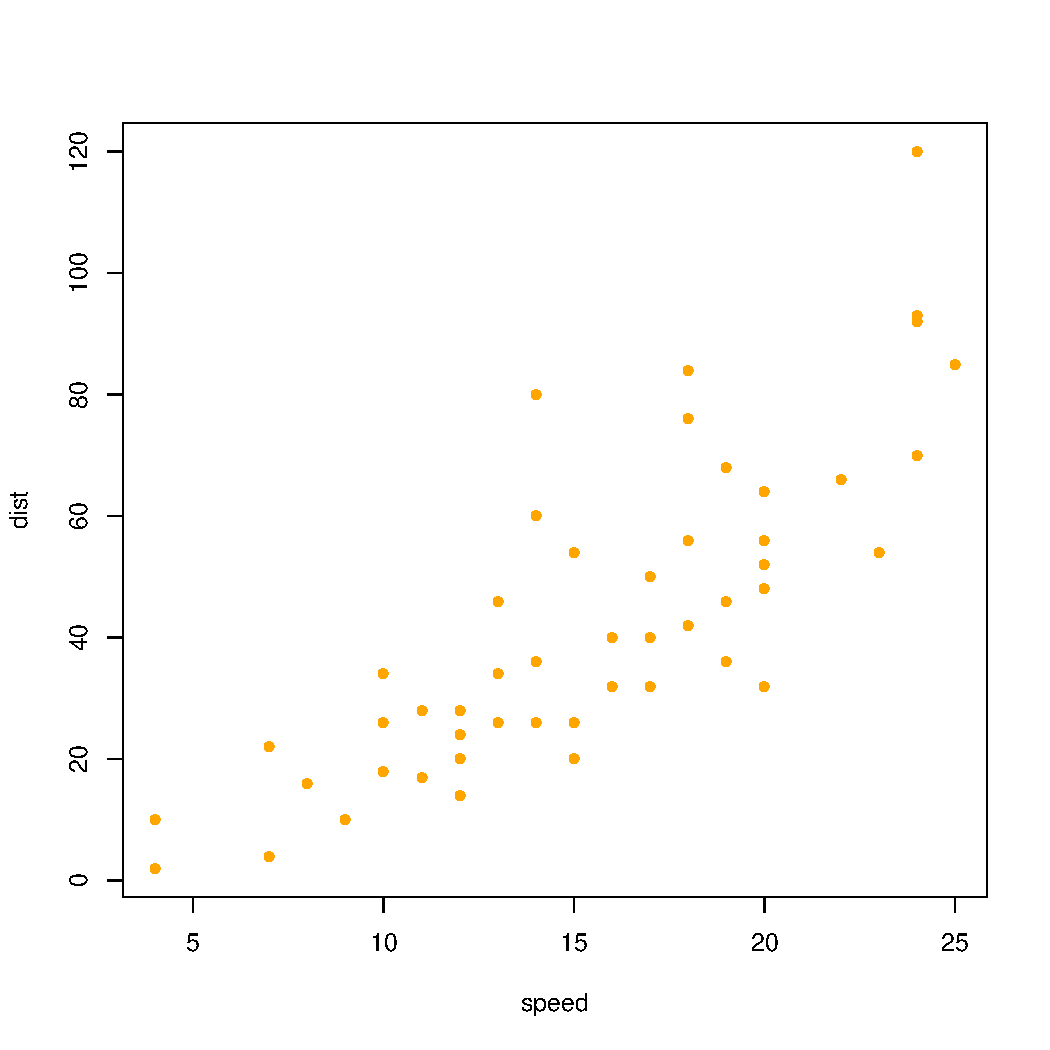
\includegraphics[width=\maxwidth]{figure/R8-1} 
\begin{kframe}\begin{alltt}
\hlstd{reco} \hlkwb{=} \hlkwd{recordPlot}\hlstd{()}
\hlcom{## Displays the inputs }
\hlstd{reco[[}\hlnum{1}\hlstd{]][[}\hlnum{4}\hlstd{]][[}\hlnum{2}\hlstd{]][[}\hlnum{2}\hlstd{]]}
\end{alltt}
\begin{verbatim}
## $x
##  [1]  4  4  7  7  8  9 10 10 10 11 11 12 12 12 12 13 13 13 13 14 14 14 14
## [24] 15 15 15 16 16 17 17 17 18 18 18 18 19 19 19 20 20 20 20 20 22 23 24
## [47] 24 24 24 25
## 
## $y
##  [1]   2  10   4  22  16  10  18  26  34  17  28  14  20  24  28  26  34
## [18]  34  46  26  36  60  80  20  26  54  32  40  32  40  50  42  56  76
## [35]  84  36  46  68  32  48  52  56  64  66  54  70  92  93 120  85
## 
## $xlab
## [1] "cars$speed"
## 
## $ylab
## [1] "cars$dist"
\end{verbatim}
\end{kframe}
\end{knitrout}

This example shows that: suppose we have a data set called \texttt{cars}, which contain two columns, the speed of the cars and the distance of travel. We have a plot which plotted the speed againist to the distance of travel. the \texttt{recordPlot()} will save this plot as an R object. As result, we can access the information of this plot. For example, the x-coordinate and the y-coordinate, or the x-label and the y-label.


There are many way for solving this problem, one possible solution will be translate the C code to R code such that as simliar as possible. The reason for doing this direct translation because: \\\\
1. It is hard to debug and track the C code.
2. It is very simple to debug the R code. If the R code is almost identical to the C code, then we can debug the R code to ensure that the R code can also provide the same result.

\subsection{standalone}
The functions that provides the persp() are huge, hence this section will only described some key step for building the functions.

\


\end{document}
